\documentclass[tikz,border=2pt]{standalone}
\usepackage{amsmath}
\usepackage[T1]{fontenc}
\usepackage{XCharter}
\usepackage[scaled=0.96]{sourcesanspro}
\usetikzlibrary{arrows.meta,calc,positioning,fit,backgrounds}
\definecolor{ink}{HTML}{222222}
\definecolor{cb}{HTML}{0072B2}
\definecolor{co}{HTML}{E69F00}
\definecolor{cs}{HTML}{56B4E9}
\newcommand{\sm}{\fontsize{6.5}{7.4}\selectfont}
\tikzset{
  every node/.style={font=\fontsize{7.2}{8.3}\selectfont, text=ink},
  layer/.style={draw=ink, rounded corners=1.6pt, line width=0.5pt, fill=cs!16, align=center, inner sep=2.2pt},
  small/.style={layer, dashed, dash pattern=on 2pt off 1.4pt, fill=white},
  turn/.style={draw=ink, line width=0.4pt, minimum size=0.26cm, inner sep=0pt},
  arr/.style={-{Stealth[length=3.2pt,width=2.6pt]}, line width=0.5pt, draw=ink},
  darr/.style={arr, densely dashed},
  edge/.style={line width=0.35pt, draw=ink!70},
  frame/.style={draw=ink!50, rounded corners=2.5pt, line width=0.4pt, inner sep=3.5pt},
  ttl/.style={font=\fontsize{7.8}{8.8}\selectfont\bfseries, anchor=west},
}
\begin{document}
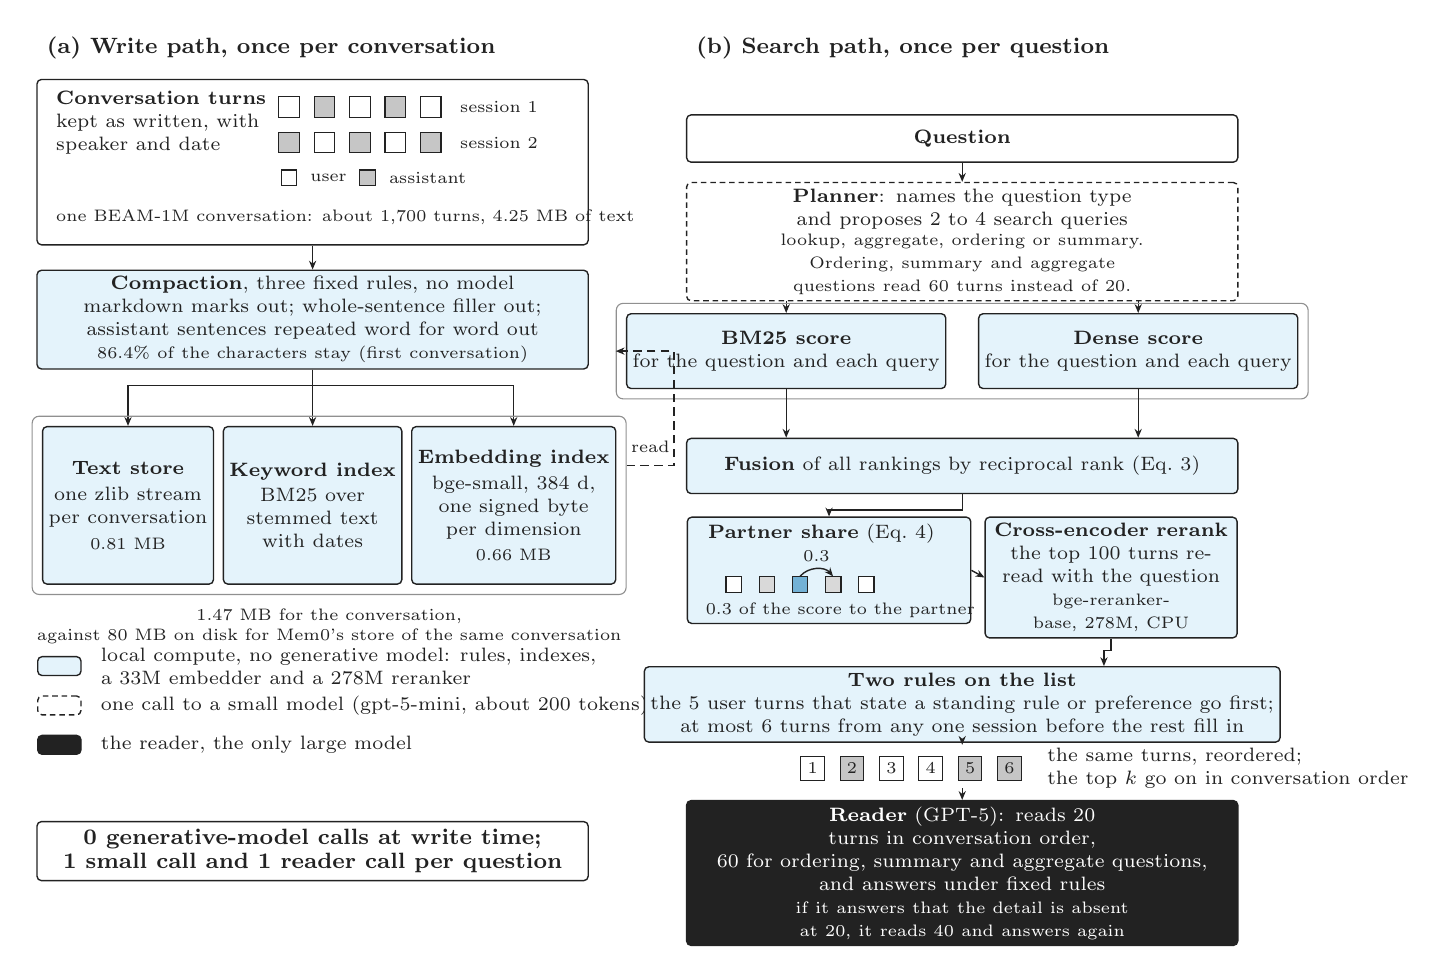
\begin{tikzpicture}[x=1cm,y=1cm]
\def\LX{3.5}
\def\RX{11.75}
\def\W{7.0}

\node[ttl] at (\LX-\W/2,1.3) {(a) Write path, once per conversation};
\node[ttl] at (\RX-\W/2,1.3) {(b) Search path, once per question};

% ================= (a) =================
\node[layer, fill=white, minimum width=\W cm, minimum height=2.1cm] (hist) at (\LX,-0.15) {};
\node[anchor=west, align=left] at (\LX-\W/2+0.12,0.35) {\textbf{Conversation turns}\\kept as written, with\\speaker and date};
\foreach \i/\c in {0/white,1/gray,2/white,3/gray,4/white} { \node[turn, fill=\c!45] at (\LX-0.3+0.45*\i,0.55) {}; }
\foreach \i/\c in {0/gray,1/white,2/gray,3/white,4/gray} { \node[turn, fill=\c!45] at (\LX-0.3+0.45*\i,0.1) {}; }
\node[anchor=west, font=\sm] at (\LX+1.75,0.55) {session 1};
\node[anchor=west, font=\sm] at (\LX+1.75,0.1) {session 2};
\node[turn, fill=white, minimum size=0.2cm] (sa) at (\LX-0.3,-0.35) {};
\node[anchor=west, font=\sm] at ($(sa.east)+(0.04,0)$) {user};
\node[turn, fill=gray!45, minimum size=0.2cm] (sb2) at (\LX+0.7,-0.35) {};
\node[anchor=west, font=\sm] at ($(sb2.east)+(0.04,0)$) {assistant};
\node[anchor=west, font=\sm] at (\LX-\W/2+0.12,-0.85) {one BEAM-1M conversation: about 1,700 turns, 4.25 MB of text};

\node[layer, minimum width=\W cm, minimum height=1.05cm, text width=6.6cm] (comp) at (\LX,-2.15) {\textbf{Compaction}, three fixed rules, no model\\markdown marks out; whole-sentence filler out; assistant sentences repeated word for word out\\{\sm 86.4\% of the characters stay (first conversation)}};
\draw[arr] (hist.south) -- (comp.north);

\node[layer, minimum width=2.15cm, minimum height=2.0cm, anchor=north east] (tx) at (\LX-1.25,-3.5) {\textbf{Text store}\\[1pt]one zlib stream\\per conversation\\[1pt]{\sm 0.81 MB}};
\node[layer, minimum width=2.15cm, minimum height=2.0cm, anchor=north] (bm) at (\LX,-3.5) {\textbf{Keyword index}\\[1pt]BM25 over\\stemmed text\\with dates};
\node[layer, minimum width=2.15cm, minimum height=2.0cm, anchor=north west] (de) at (\LX+1.25,-3.5) {\textbf{Embedding index}\\[1pt]bge-small, 384 d,\\one signed byte\\per dimension\\[1pt]{\sm 0.66 MB}};
\draw[arr] (comp.south) -- ++(0,-0.2) -| (tx.north);
\draw[arr] (comp.south) -- ++(0,-0.2) -| (bm.north);
\draw[arr] (comp.south) -- ++(0,-0.2) -| (de.north);
\node[frame, fit=(tx)(bm)(de)] (mem) {};
\node[anchor=north, font=\sm, align=center] at ($(mem.south)+(0,-0.05)$) {1.47 MB for the conversation,\\against 80 MB on disk for Mem0's store of the same conversation};

% legend
\node[layer, minimum width=0.55cm, minimum height=0.24cm, anchor=west] (l1) at (\LX-\W/2,-6.55) {};
\node[anchor=west, align=left] at ($(l1.east)+(0.12,0)$) {local compute, no generative model: rules, indexes,\\a 33M embedder and a 278M reranker};
\node[small, minimum width=0.55cm, minimum height=0.24cm, anchor=west] (l2) at (\LX-\W/2,-7.05) {};
\node[anchor=west] at ($(l2.east)+(0.12,0)$) {one call to a small model (gpt-5-mini, about 200 tokens)};
\node[layer, fill=ink, minimum width=0.55cm, minimum height=0.24cm, anchor=west] (l3) at (\LX-\W/2,-7.55) {};
\node[anchor=west] at ($(l3.east)+(0.12,0)$) {the reader, the only large model};

% ================= (b) =================
\node[layer, fill=white, minimum width=\W cm, minimum height=0.6cm] (qu) at (\RX,0.15) {\textbf{Question}};
\node[small, minimum width=\W cm, minimum height=0.8cm, anchor=north, text width=6.6cm] (pl) at (\RX,-0.4) {\textbf{Planner}: names the question type and proposes 2 to 4 search queries\\{\sm lookup, aggregate, ordering or summary.\\Ordering, summary and aggregate questions read 60 turns instead of 20.}};
\draw[arr] (qu.south) -- (pl.north);

\node[layer, minimum width=3.2cm, minimum height=0.95cm, anchor=east] (sb) at (\RX-0.2,-2.55) {\textbf{BM25 score}\\for the question and each query};
\node[layer, minimum width=3.2cm, minimum height=0.95cm, anchor=west] (sd) at (\RX+0.2,-2.55) {\textbf{Dense score}\\for the question and each query};
\draw[arr] (pl.south -| sb.north) -- (sb.north);
\draw[arr] (pl.south -| sd.north) -- (sd.north);
\node[frame, fit=(sb)(sd)] (scr) {};
\draw[darr] (mem.east |- 0,-4.0) -- ++(0.6,0) node[above left=1pt and -2pt, font=\sm] {read} |- (scr.west);

\node[layer, minimum width=\W cm, minimum height=0.7cm, anchor=north] (fu) at (\RX,-3.65) {\textbf{Fusion} of all rankings by reciprocal rank (Eq.~3)};
\draw[arr] (sb.south) -- (sb.south |- fu.north);
\draw[arr] (sd.south) -- (sd.south |- fu.north);

\node[layer, minimum width=3.6cm, minimum height=1.35cm, anchor=north west] (pr) at (\RX-\W/2,-4.65) {};
\node[anchor=west] at ($(pr.north west)+(0.15,-0.22)$) {\textbf{Partner share} (Eq.~4)};
\foreach \i/\c in {0/white,1/gray,2/white,3/gray,4/white} { \node[turn, minimum size=0.2cm, fill=\c!30] (c\i) at ($(pr.south west)+(0.6+0.42*\i,0.5)$) {}; }
\node[turn, minimum size=0.2cm, fill=cb!55] at (c2) {};
\draw[arr] (c2.north) to[bend left=50] node[above=-1pt, font=\sm] {0.3} (c3.north);
\node[font=\sm, anchor=west] at ($(pr.south west)+(0.12,0.17)$) {0.3 of the score to the partner};
\node[layer, minimum width=3.2cm, minimum height=1.35cm, anchor=north east, text width=3.0cm] (rr) at (\RX+\W/2,-4.65) {\textbf{Cross-encoder rerank}\\the top 100 turns re-read with the question\\{\sm bge-reranker-base, 278M, CPU}};
\draw[arr] (fu.south) -- ++(0,-0.2) -| (pr.north);
\draw[arr] (pr.east) -- (rr.west);

\node[layer, minimum width=\W cm, minimum height=0.9cm, anchor=north] (ru) at (\RX,-6.55) {\textbf{Two rules on the list}\\the 5 user turns that state a standing rule or preference go first;\\at most 6 turns from any one session before the rest fill in};
\draw[arr] (rr.south) -- ++(0,-0.15) -| ($(ru.north)+(1.8,0)$);

% output: ranked list
\coordinate (o0) at (\RX-1.9,-7.85);
\draw[arr] (ru.south) -- (\RX,-7.55);
\foreach \i/\c in {0/white,1/gray,2/white,3/white,4/gray,5/gray} { \node[turn, fill=\c!45, minimum size=0.3cm] (r\i) at ($(o0)+(0.5*\i,0)$) {}; }
\foreach \i in {0,...,5} { \node[font=\sm] at (r\i) {\pgfmathparse{int(\i+1)}\pgfmathresult}; }
\node[anchor=west, align=left] at ($(r5.east)+(0.2,0)$) {the same turns, reordered;\\the top $k$ go on in conversation order};

% reader
\node[layer, fill=ink, text=white, minimum width=\W cm, minimum height=0.85cm, anchor=north, align=center, text width=6.6cm] (rd) at (\RX,-8.25) {\textbf{Reader} (GPT-5): reads 20 turns in conversation order,\\60 for ordering, summary and aggregate questions,\\and answers under fixed rules\\{\sm\color{white}if it answers that the detail is absent at 20, it reads 40 and answers again}};
\draw[arr] (\RX,-8.1) -- (rd.north);
% banner
\node[layer, fill=white, minimum width=\W cm, minimum height=0.75cm, align=center, text width=6.4cm, font=\bfseries\fontsize{7.8}{8.8}\selectfont] (zero) at (\LX,-8.9) {0 generative-model calls at write time;\\1 small call and 1 reader call per question};
\end{tikzpicture}
\end{document}
